\documentclass[11pt,letterpaper,titlepage]{article}

%================== Document nomenclature
\newcommand{\DOCSUBJT}{Personal Notes: }   %Put document subject here
\newcommand{\DOCTITLE}{                      %Put document title here
    One dimensional neutron transport
}       
\newcommand{\DOCDATE} {March, 2019}         %Put document date here
\newcommand{\DOCREV}  {Rev 1.00}             %Put revision number here

%================== Misc Settings
\usepackage{fancyhdr}
\usepackage[left=0.75in, right=0.75in, bottom=1.0in]{geometry}
\usepackage{lastpage}
\usepackage{titleref}
\usepackage{booktabs}
\usepackage{appendix}

\appendixtitleon
\appendixtitletocon

\makeatletter

%================== List of figures and tables mods
\usepackage{tocloft}
\usepackage[labelfont=bf]{caption}

\renewcommand{\cftfigpresnum}{Figure\ }
\renewcommand{\cfttabpresnum}{Table\ }

\newlength{\mylenf}
\settowidth{\mylenf}{\cftfigpresnum}
\setlength{\cftfignumwidth}{\dimexpr\mylenf+1.5em}
\setlength{\cfttabnumwidth}{\dimexpr\mylenf+1.5em}



%=================== Graphics
\usepackage{graphicx}
\usepackage[breakwords]{truncate}
\usepackage{float}
\usepackage{array}
\usepackage{amsmath}
\usepackage{mdframed}
\usepackage{fancyvrb}
\usepackage{float}
\usepackage{cancel}
\usepackage{amssymb}
\graphicspath{ {images/} }
\usepackage[usenames,dvipsnames,svgnames,table]{xcolor}
\usepackage[defaultlines=2,all]{nowidow}
\usepackage{listings}
\usepackage{color}
\definecolor{Brown}{cmyk}{0,0.81,1,0.60}
\definecolor{OliveGreen}{cmyk}{0.64,0,0.95,0.40}
\definecolor{CadetBlue}{cmyk}{0.62,0.57,0.23,0}
\usepackage{pdflscape}
\usepackage{relsize}
\usepackage{verbatim}
\usepackage{tabto}
%\usepackage{upgreek}
\usepackage{enumitem}
%\usepackage{MnSymbol}% http://ctan.org/pkg/mnsymbol

%=================== Big cdot
\newcommand*\bigcdot{\mathpalette\bigcdot@{.5}}
\newcommand*\bigcdot@[2]{\mathbin{\vcenter{\hbox{\scalebox{#2}{$\m@th#1\bullet$}}}}}

%=================== Settings
\renewcommand{\baselinestretch}{1.2}
\definecolor{gray}{rgb}{0.4 0.4 0.4}
\newcommand{\stimes}{{\times}}
\newcommand{\half}{\frac{1}{2}}

%================== Code syntax highlighting
\lstset{language=C++,
    frame=ltrb,
    framesep=2pt,
    basicstyle=\linespread{0.8} \small,
    keywordstyle=\ttfamily\color{OliveGreen},
    identifierstyle=\ttfamily\color{CadetBlue}\bfseries,
    commentstyle=\color{Brown},
    stringstyle=\ttfamily,
    showstringspaces=true,
    tabsize=2,}


%================== Section numbers with equation numbers
\numberwithin{equation}{section}

%================== Short \to arrow
\setlength{\medmuskip}{0mu}
%\newcommand{\tos}[1][3pt]{\mathrel{%
%   \hbox{\rule[\dimexpr\fontdimen22\textfont2-.2pt\relax]{#1}{.4pt}}%
%   \mkern-4mu\hbox{\usefont{U}{lasy}{m}{n}\symbol{41}}}}

\newcommand{\beq}{\begin{equation*}
\begin{aligned}}
\newcommand{\eeq}{\end{aligned}
\end{equation*}}

\newcommand{\beqn}{\begin{equation}
	\begin{aligned}}
\newcommand{\eeqn}{\end{aligned}
	\end{equation}}

\setlength\parindent{0pt}



\begin{document}
    
    \begin{titlepage}
        \pagestyle{fancy}
        \vspace*{1.0cm}
        \centering
        \vspace{1cm}
        \vspace{.25cm}
        {\Large\bfseries  \DOCSUBJT \par} 
        {\Large\bfseries \DOCTITLE  \par}
        \vspace{1cm}
        {\Large \DOCDATE \par}
        \vspace{1.0cm}
        {\Large Jan Vermaak \par}
        {\Large \DOCREV \par}
        
    \end{titlepage}	
    
    
    \pagestyle{fancy}
    \rfoot{Page \thepage \ of \pageref{LastPage}}
    \cfoot{}
    \lfoot{\truncate{14cm}{\DOCTITLE}}
    \rhead{}
    \chead{\currentname}
    \lhead{}
    \renewcommand{\footrulewidth}{0.4pt}
    
    \begin{comment}
    \tableofcontents
    \addtocontents{toc}{~\hfill\textbf{Page}\par}
    
    \listoffigures
    \listoftables
    
    \end{comment}
    \chead{Contents}	
    
    %#########################################################################
\newpage 
\chead{The 1D neutron transport equation}
\section{The one-dimensional neutron transport equation}
We start with the three dimensional multi-group transport equation

\begin{equation} \label{eq:multiGroupNTE}
\begin{aligned}
&\biggr(\Omega\nabla +\Sigma_{tg} (r)\biggr)  \Psi_g (r,\Omega)
= \sum_{\ell=0}^{\infty}\sum_{m=-\ell}^{\ell} Y_{\ell m}(\Omega)
\biggr[ \sum_{g'=0}^{G-1}
\Sigma_{sl,g'{\to}g} (r)
  \phi_{g'\ell m} (r)
\biggr]
+  S_g (r,\Omega).
\end{aligned}
\end{equation}

Here the spherical harmonics are given by

\beqn
Y_{\ell m} (\theta, \varphi )=
\begin{cases}
 \sqrt(2)\sqrt{ \frac{(2\ell + 1)}{4\pi}   \frac{(\ell-|m|)!}{(\ell+|m|)!}}P_{\ell}^{|m|}(\cos\theta)sin\ {|m|\varphi}
& \text{if } m < 0 \\
\sqrt{ \frac{(2\ell + 1)}{4\pi}} P_{\ell}^{m}(cos\theta) & \text{if } m = 0 \\
 \sqrt(2)\sqrt{ \frac{(2\ell + 1)}{4\pi}   \frac{(\ell-m)!}{(\ell+m)!}}P_{\ell}^{m}(\cos\theta)cos\ {m\varphi}
& \text{if } m \ge 0 \\
\end{cases}
\eeqn

We recall from the expansion of the angular flux into spherical harmonics that 

\beq
\phi_{g'\ell m}(r) = \int_0^{2\pi}\int_{-1}^1 \Psi_g(r,\mu,\varphi).Y_{\ell m}(\mu,\varphi).d\mu.d\varphi
\eeq 

In one dimension the angular flux will not be a function of $\varphi$ and therefore when we rearrange the integration we get

\beq
\phi_{g'\ell m}(r) &= \int_{-1}^1 \Psi_g(r,\mu,\cancel{\varphi})\int_0^{2\pi}Y_{\ell m}(\mu,\varphi).d\varphi.d\mu \\
&=
\begin{cases}
0, &\text{ if } m \ne \ell, \\
\sqrt{ \frac{(2\ell + 1)}{4\pi}} \int_{-1}^1 \Psi_{g'}(r,\mu)P_{\ell}^{0}(\mu).d\mu & \text{if } m = 0 \\
\end{cases}
\eeq

and from the fundamental definition of the associated Legendre Polynomials we have $P_\ell^0 = P_\ell$ and hence equation \ref{eq:multiGroupNTE} reduces to

\begin{equation} 
\begin{aligned}
&\biggr(\Omega\nabla +\Sigma_{tg} (r)\biggr)  \Psi_g (r,\Omega)
= \sum_{\ell=0}^{\infty}\frac{2\ell+1}{4\pi}P_\ell(\mu)
\biggr[ \sum_{g'=0}^{G-1}
\Sigma_{sl,g'{\to}g} (r)
  \phi_{g'\ell} (r)
\biggr]
+  S_g (r,\Omega).
\end{aligned}
\end{equation}

where

\beq 
\phi_{g'\ell}(r) = \int_{-1}^1 \Psi_{g'}(r,\mu)P_\ell(\mu).d\mu 
\eeq 

The final step is to integrate over azimuthal angle where we first define

\beq 
\Psi_g(r,\mu) &= \int_0^{2\pi}\Psi_g(r,\Omega).d\varphi \\
S_g (r,\mu) &= \int_0^{2\pi} S_g(r,\Omega).d\varphi
\eeq 

and note that no term in the scattering source is dependent on $\varphi$ therefore the integration over angle gives
\begin{equation} 
\begin{aligned}
& \int_0^{2\pi}
\biggr(\Omega\nabla +\Sigma_{tg} (r)\biggr)  
\Psi_g (r,\Omega)
.d\varphi 
=  \int_0^{2\pi}
\biggr(
\sum_{\ell=0}^{\infty}\frac{2\ell+1}{4\pi}P_\ell(\mu)
\biggr[ \sum_{g'=0}^{G-1}
\Sigma_{sl,g'{\to}g} (r)
  \phi_{g'\ell} (r)
\biggr]\biggr).d\varphi 
+  
 \int_0^{2\pi}
S_g (r,\Omega)
.d\varphi 
.
\end{aligned}
\end{equation}

\begin{equation} 
\begin{aligned}
&\biggr(\mu\frac{\partial}{\partial x} +\Sigma_{tg} (r)\biggr)  \Psi_g (r,\mu)
= \sum_{\ell=0}^{L}\frac{2\ell+1}{2}P_\ell(\mu)
\biggr[ \sum_{g'=0}^{G-1}
\Sigma_{sl,g'{\to}g} (r)
  \phi_{g'\ell} (r)
\biggr]
+  S_g (r,\mu).
\end{aligned}
\end{equation}

Note that we also truncated the scattering term expansion to $L$ instead of infinity. We now introduce the Discrete Ordinates method by approximating the integration over angle with a quadrature rule. To this end we can write

\beq
\phi_{g'\ell} (r)= \int_{-1}^1 \Psi_{g'}(r,\mu)P_\ell(\mu).d\mu \approx 
\sum_{n=0}^{N_a-1} w_n \Psi_{g'}(r,\mu_n)P_\ell(\mu_n)
\eeq 

and colocate discrete angles with the angles arising from this quadrature to obtain

\begin{equation} 
\begin{aligned}
&\biggr(\mu\frac{\partial}{\partial x} +\Sigma_{tg} (r)\biggr)  \Psi_g (r,\mu_n)
= \sum_{\ell=0}^{L}\frac{2\ell+1}{2}P_\ell(\mu_n)
\biggr[ \sum_{g'=0}^{G-1}
\Sigma_{sl,g'{\to}g} (r)
  \sum_{n=0}^{N_a-1} w_n P_\ell(\mu_n)\Psi_{g'}(r,\mu_n)
\biggr]
+  S_g (r,\mu_n).
\end{aligned}
\end{equation}

As a simplification we write $\Psi_g(r,\mu_n)$ as $\Psi_{gn}$ and do the same for all terms in this form to get

\begin{equation} 
\begin{aligned}
&\biggr(\mu\frac{\partial}{\partial x} +\Sigma_{tg} \biggr)  \Psi_{gn}
= \sum_{\ell=0}^{L}\frac{2\ell+1}{2}P_\ell(\mu_n)
\biggr[ \sum_{g'=0}^{G-1}
\Sigma_{sl,g'{\to}g} 
  \sum_{n=0}^{N_a-1} w_n P_\ell(\mu_n)\Psi_{g'n}
\biggr]
+  S_{gn}.
\end{aligned}
\end{equation}


We now perform a series of algebraic manipulations to obtain an operator form. To this end we first define the angular flux for group $g'$ as

\beq 
\mathbf{\Psi}_{g'}  = 
\begin{bmatrix}
\Psi_{g'0} \\
\vdots \\
\Psi_{g'(N_a-1)}
\end{bmatrix}
\eeq 

this is a \textbf{sub-vector} of size $N_a \stimes 1$ which gets multiplied by a vector $\mathbf{D}_{\ell,g}$ of transpose size $1\stimes N_a$ defined as

\beq 
\mathbf{D}_{\ell,g}  = 
\begin{bmatrix}
w_0 P_{\ell}(\mu_n) &\hdots &w_{N_a-1} P_{\ell}(\mu_n) \\
\end{bmatrix}
\eeq 

The multiplication $\mathbf{D}_{\ell,g}\mathbf{\Psi}_{g'}$  results in a $1\stimes 1$ scalar value and therefore our equation is now

\begin{equation} 
\begin{aligned}
&\biggr(\mu\frac{\partial}{\partial x} +\Sigma_{tg} \biggr)  \Psi_{gn}
= \sum_{\ell=0}^{L}\frac{2\ell+1}{2}P_\ell(\mu_n)
\biggr[ \sum_{g'=0}^{G-1}
\Sigma_{sl,g'{\to}g} 
\mathbf{D}_{\ell,g} \mathbf{\Psi}_{g'}
\biggr]
+  S_{gn}.
\end{aligned}
\end{equation}

We now define the full angular flux vector $\mathbf{\Psi}$ of size $(N_a\stimes G)\stimes 1$ 

\beq 
\mathbf{\Psi} = 
\begin{bmatrix}
\mathbf{\Psi}_{0} \\ 
\vdots \\
\mathbf{\Psi}_{G-1}
\end{bmatrix}
\eeq 

And we define the matrix $\mathbf{D}_\ell$ of size $G\stimes (N_a \stimes G)$

\beq 
\mathbf{D}_{\ell}  = 
\begin{bmatrix}
\mathbf{D}_{\ell,0}  & \hdots & 0 \\
\vdots &\ddots &\vdots \\
0 & \hdots &\mathbf{D}_{\ell,G-1} 
\end{bmatrix}
\eeq 


The matrix-vector multiplication $\mathbf{D}_\ell \mathbf{\Psi}$ will result in a vector with size $G\stimes 1$ after which we define scattering moment vector $\mathbf{S}_\ell$ of size $G\stimes 1$

\beq
\mathbf{S}_\ell= 
\begin{bmatrix}
\Sigma_{s\ell,0{\to}g} &\hdots &\Sigma_{s\ell,(G-1){\to}g} \\
\end{bmatrix}
\eeq 

The vector multiplication $\mathbf{S}_\ell \mathbf{D}_\ell \mathbf{\Psi}$ will result a value of size $1\stimes 1$ and equation then is

\begin{equation} 
\begin{aligned}
&\biggr(\mu\frac{\partial}{\partial x} +\Sigma_{tg} \biggr)  \Psi_{gn}
= \sum_{\ell=0}^{L}\frac{2\ell+1}{2}P_\ell(\mu_n)
\mathbf{S}_\ell \mathbf{D}_\ell \mathbf{\Psi}
+  S_{gn}.
\end{aligned}
\end{equation}

Finally we define the moment to discrete operator $\mathbf{M}_n$ which has a size $1\stimes (L+1)$ as

\beq
\mathbf{M}_n = 
\begin{bmatrix}
\frac{2(0)+1}{2} P_0(\mu_n) &\hdots &\hdots &\frac{2(L)+1}{2} P_L(\mu_n)\\
\end{bmatrix}
\eeq 

as well as the vector

\beq 
\mathbf{SD}  = 
\begin{bmatrix}
\mathbf{S}_0 \mathbf{D}_0 \mathbf{\Psi}\\
\vdots \\
\mathbf{S}_L \mathbf{D}_L \mathbf{\Psi}\\
\end{bmatrix}
\eeq 

And when we put all of this together we get the equation

\begin{equation} 
\begin{aligned}
&\biggr(\mu\frac{\partial}{\partial x} +\Sigma_{tg} \biggr)  \Psi_{gn}
= \mathbf{M}_n
\mathbf{S} \mathbf{D} \mathbf{\Psi}
+  S_{gn}.
\end{aligned}
\end{equation}

where we can seperate $\mathbf{SD}$ as $\mathbf{D}$ with size $((L+1).G)\stimes (N_a . G)$
\beq 
\mathbf{D}  = 
\begin{bmatrix}
\mathbf{D}_0 \\
\vdots \\
\mathbf{D}_L
\end{bmatrix}
\eeq 

and $\mathbf{S}$ with size $(L+1) \stimes ((L+1).G)$

\beq
\mathbf{S}= 
\begin{bmatrix}
\mathbf{S}_0     &\hdots &0 \\
\vdots               &\ddots &\vdots \\
0                      &\hdots &\mathbf{S}_L
\end{bmatrix}
\eeq 

Auditing this exercise from right to left we have

\beq 
\mathbf{D}^{((L+1) .G)\stimes (N_a . G)}    \mathbf{\Psi}^{(N_a.G) \stimes 1}
&\to (\mathbf{D\Psi })^{((L+1) .G)\stimes 1} \\
\mathbf{S}^{(L+1)  \stimes ((L+1) .G)}(\mathbf{D\Psi })^{((L+1) .G)\stimes 1} 
&\to (\mathbf{SD\Psi})^{(L+1) \stimes 1} \\
\mathbf{M}_n^{1\stimes (L+1)}(\mathbf{SD\Psi})^{(L+1) \stimes 1} 
&\to (\mathbf{M}_n \mathbf{SD\Psi})^{1\stimes 1}
\eeq 
\newline
Additionally we can now define the $\mathbf{L}$ operator, but not develop it, to have the operator form of the neutron transport equation

\beqn \label{eq:NTEoperatorform}
\mathbf{L \Psi} = \mathbf{MSD\Psi} + \mathbf{S}
\eeqn 








\newpage
\section{PWLD Finite Element application}
The finite element method can be applied to the multigroup form of the transport equation by multiplying by a trial function, $\varphi_i(x)$, and integrating over the volume of the trial space. 

\subsection{Applying a trial space}

First consider the following form of the equation

\begin{equation*} 
\begin{aligned}
\mu\frac{\partial \Psi_{gn}}{\partial x} 
+\Sigma_{tg}  \Psi_{gn}
&= Q_{s,gn}
+  S_{gn}
\end{aligned}
\end{equation*}
where
\begin{equation*} 
\begin{aligned}
Q_{s,gn} & = \sum_{\ell=0}^{L}\frac{2\ell+1}{2}P_\ell(\mu)
\biggr[ \sum_{g'=0}^{G-1}
\Sigma_{sl,g'{\to}g} 
  \phi_{g'\ell} 
\biggr]
\end{aligned}
\end{equation*}

We now multiply by $\varphi_i$ (a trial space function) and integrate over the volume of the trial space

\begin{equation*} 
\begin{aligned}
\int \varphi_i.\mu.\frac{\partial \Psi_{gn}}{\partial x} .dx
+\int \varphi_i.\Sigma_{tg}  \Psi_{gn}.dx
&= \int \varphi_i \biggr[Q_{s,gn}
+  S_{gn} \biggr].dx
\end{aligned}
\end{equation*}

next we apply integration by parts to the first term by first noting

\begin{equation*} 
\begin{aligned}
\frac{\partial (\varphi_i.\mu\Psi_{gn})}{\partial x} 
= \frac{\partial \varphi_i}{\partial x} . \mu\Psi_{gn} 
+ \varphi_i.\mu.\frac{\partial \Psi_{gn}}{\partial x}
\end{aligned}
\end{equation*}

therefore

\begin{equation*} 
\begin{aligned}
\int \frac{\partial (\varphi_i.\mu\Psi_{gn})}{\partial x}  .dx
-\int  \frac{\partial \varphi_i}{\partial x} . \mu\Psi_{gn}  .dx
+\int \varphi_i.\Sigma_{tg}  \Psi_{gn}.dx
&= \int \varphi_i \biggr[Q_{s,gn}
+  S_{gn} \biggr].dx.
\end{aligned}
\end{equation*}

Now from the 3D Gauss Divergence theorem, which states

\beq 
\int_V \nabla f = \int_S \hat{n}\cdot f .dA,
\eeq 

we get

\beq
(\varphi_i.\mu\tilde{\Psi}_{gn})
-\int  \frac{\partial \varphi_i}{\partial x} . \mu\Psi_{gn}  .dx
+\int \varphi_i.\Sigma_{tg}  \Psi_{gn}.dx
&= \int \varphi_i \biggr[Q_{s,gn}
+  S_{gn} \biggr].dx.
\eeq 

where we define an upwinding scheme on $\tilde{\Psi}_{gn}$ as

\beq
\tilde{\Psi}_{gn} = 
\begin{cases}
\Psi_{gn} \quad \quad & \text{ if } \hat{n}\cdot \mu > 0, \\
\Psi_{gn,upwind} \quad \quad & \text{ if } \hat{n}\cdot \mu < 0,
\end{cases}
\eeq 

We now apply integration by parts again on the second term

\beq
(\varphi_i.\hat{n} \cdot \mu\tilde{\Psi}_{gn})
-\int  \frac{\partial (\varphi_i.\mu\Psi_{gn})}{\partial x}  .dx
+\int  \varphi_i.\mu.\frac{\partial \Psi_{gn}}{\partial x}.dx
+\int \varphi_i.\Sigma_{tg}  \Psi_{gn}.dx
&= \int \varphi_i \biggr[Q_{s,gn}
+  S_{gn} \biggr].dx.
\eeq 

and apply Gauss' divergence theorem again

\beq
(\varphi_i.\hat{n}\cdot \mu\tilde{\Psi}_{gn} )
-(\varphi_i.\hat{n}\cdot \mu\Psi_{gn})
+\int  \varphi_i.\mu.\frac{\partial \Psi_{gn}}{\partial x}.dx
+\int \varphi_i.\Sigma_{tg}  \Psi_{gn}.dx
&= \int \varphi_i \biggr[Q_{s,gn}
+  S_{gn} \biggr].dx.
\eeq 

We can now rearrange the terms from where we obtain the weak form of the equation

\beqn
\varphi_i.\hat{n}\cdot \mu(\tilde{\Psi}_{gn}-\Psi_{gn})
+\int  \varphi_i.\mu.\frac{\partial \Psi_{gn}}{\partial x}.dx
+\int \varphi_i.\Sigma_{tg}  \Psi_{gn}.dx
&= \int \varphi_i \biggr[Q_{s,gn}
+  S_{gn} \biggr].dx 
\eeqn 


\subsection{Expanding the unknowns into bases}
We now expand the angular flux into basis functions, $b_j$ as

\beq
\Psi_{gn} = \sum_{j=0}^{N-1} \Psi_{gn,j} b_j
\eeq 

and when we insert this into the weak form we get

\beq
\sum_{j=0}^{N-1}  \biggr[
\varphi_i.\mu(\tilde{\Psi}_{gn}-\Psi_{gn,j}b_j)
+\Psi_{gn,j}\int  \varphi_i.\mu.\frac{\partial b_j}{\partial x}.dx
+\Psi_{gn,j} \int \varphi_i.\Sigma_{tg} b_j.dx
\biggr]
&= \int \varphi_i \biggr[Q_{s,gn}
+  S_{gn} \biggr].dx\\
\eeq 

and after manipulation

\beqn \label{eq:FEMnodei} 
\sum_{j=0}^{N-1} \Psi_{gn,j} &\biggr[
-(\mu \varphi_i.  b_j )
+\mu \int  \varphi_i.\frac{\partial b_j}{\partial x}.dx
+ \Sigma_{tg}\int \varphi_i. b_j.dx
\biggr]\\
&= \biggr[Q_{s,gn}
+  S_{gn} \biggr]\int \varphi_i .dx
- \sum_{j=0}^{N-1} \tilde{\Psi}_{gn,j} (\mu \varphi_i.  b_j )
\eeqn

This equation is valid for each node $i$ of a given element and for integratable trial and basis functions it results in a linear equation for each node. Consequently we can construct a linear system for each cell using this equation. 

\newpage
\subsection{Defining the trial- and basis functions}
Up to now we have not defined either the trial functions $\varphi_i$ or the basis functions $b_j$. For the piecewise linear method we can firstly choose to use the same functions for both the trial and basis functions, making the method a Galerkin method, and secondly we can use piecewise linear functions defined on a reference element defined on $\xi\in[-1,1]$ as

\beq
\varphi(\xi) = b(\xi) = 
\begin{cases}
-\frac{1}{2}\xi+\frac{1}{2}    \quad \quad &\text{ supported on } \xi=-1\\
+\frac{1}{2}\xi+\frac{1}{2}    \quad \quad &\text{ supported on } \xi=1\\
\end{cases}
\eeq 

or 

\beq
N_0(\xi) &= -\frac{1}{2}\xi+\frac{1}{2} \\
N_1(\xi) &= +\frac{1}{2}\xi+\frac{1}{2}
\eeq 
\newline
A graphical representation of these shape functions is shown in the figure below.
\begin{figure}[H]
\centering
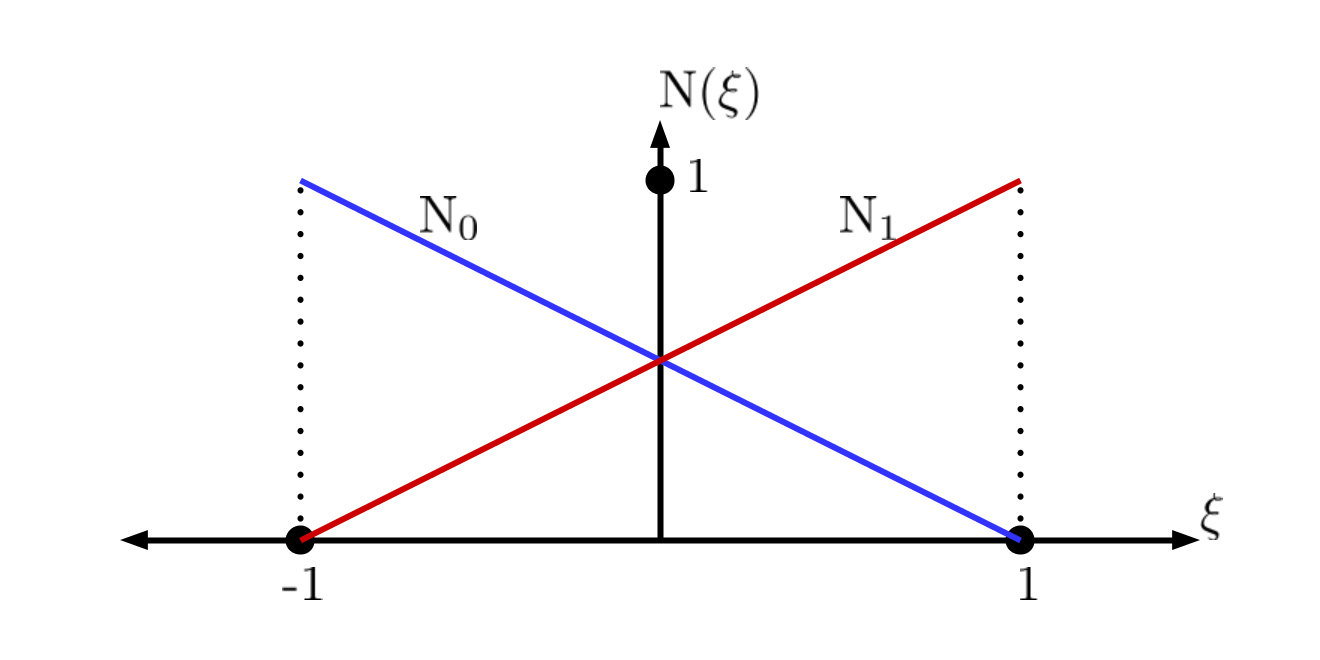
\includegraphics[width=0.5\linewidth]{images/ShapeFunctions.png}
\caption{Piecewise Linear shape functions used for the finite element trial space and basis expansion.}
\label{fig:shapefunctions}
\end{figure}


In one dimension we can compute any integral of a function $f$, defined on an element, as a transformation of the integral of $g$ over the reference element by first noting

\beq
x &= N_0 x_i + N_1 x_{i+1} \\
 &= (-\frac{1}{2}\xi+\frac{1}{2}) x_i + (+\frac{1}{2}\xi+\frac{1}{2})x_{i+1} \\
 \therefore
 x &= \frac{1}{2}\biggr( x_i + x_{i+1} \biggr) 
 + \frac{1}{2}\xi \biggr( x_{i+1}-x_i    \biggr)
\eeq 
Taking the derivate we get 

\beq
\frac{dx}{d\xi} = \frac{1}{2}\biggr( x_{i+1}-x_i    \biggr)
\eeq 

Then for an integral we have
\beq
\int_{x_i}^{x_{i+1}} f(x).dx =\frac{x_{i+1}-x_i}{2}\int_{-1}^{+1} g(\xi).d\xi.
\eeq

With this machinery in place we can easily compute the integrals of $\varphi_i$ and the product $\varphi_i.b_j$, however, the integral of a derivative term needs some modification because

\beq
\frac{\partial f}{\partial x} = \frac{\partial f}{\partial \xi} 
.\frac{\partial \xi}{\partial x}
\eeq 

but fortunately for the one dimensional case 

\beq
\frac{\partial \xi}{\partial x}  = \frac{2}{x_{i+1}-x_i}.
\eeq 

We can now proceed to calculate the integrals which is detailed in the appendix and summarized here

\beqn
&\int_{x_i}^{x_{i+1}} \varphi_0 .dx  = \frac{h}{2}  \quad \quad
&&\int_{x_i}^{x_{i+1}} \varphi_1 .dx  = \frac{h}{2} \\
\dots \\
&\int_{x_i}^{x_{i+1}} \varphi_0 b_0.dx =\frac{h}{3}
&&\int_{x_i}^{x_{i+1}} \varphi_0 b_1.dx =\frac{h}{6} \\
&\int_{x_i}^{x_{i+1}} \varphi_1 b_0.dx =\frac{h}{6} 
&&\int_{x_i}^{x_{i+1}} \varphi_1 b_1.dx =\frac{h}{3} \\
\dots \\
&\int_{x_i}^{x_{i+1}} \varphi_0.\frac{\partial b_0}{\partial x}.dx = -\frac{1}{2}
&&\int_{x_i}^{x_{i+1}} \varphi_0.\frac{\partial b_1}{\partial x}.dx = \frac{1}{2} \\
&\int_{x_i}^{x_{i+1}} \varphi_1.\frac{\partial b_0}{\partial x}.dx = -\frac{1}{2} 
&&\int_{x_i}^{x_{i+1}} \varphi_1.\frac{\partial b_1}{\partial x}.dx = \frac{1}{2} \\
\dots \\
&\int_{x_i}^{x_{i+1}} \frac{\partial \varphi_0}{\partial x}.\frac{\partial b_0}{\partial x}.dx = \frac{1}{h}
&&\int_{x_i}^{x_{i+1}} \frac{\partial \varphi_0}{\partial x}.\frac{\partial b_1}{\partial x}.dx =- \frac{1}{h}\\
&\int_{x_i}^{x_{i+1}} \frac{\partial \varphi_1}{\partial x}.\frac{\partial b_0}{\partial x}.dx = -\frac{1}{h} 
&&\int_{x_i}^{x_{i+1}} \frac{\partial \varphi_1}{\partial x}.\frac{\partial b_1}{\partial x}.dx = \frac{1}{h} \\
\eeqn


\newpage
\section{Simplified 1D, single group isotropic scattering algorithm}
For a single energy group we have the simplification that the summation over energy groups does not feature and therefore our transport equation reduces to

\begin{equation} 
\begin{aligned}
&\biggr(\mu\frac{\partial}{\partial x} +\Sigma_{t} (r)\biggr)  \Psi (r,\mu)
= \sum_{\ell=0}^{L}\frac{2\ell+1}{2}P_\ell(\mu)
\Sigma_{s\ell} (r)
  \phi_{\ell} (r)
\biggr]
+  S (r,\mu).
\end{aligned}
\end{equation}

Additionally we assume isotropic scattering and an isotropic source. For the scattering moments we recall that 
\beq 
\Sigma_{s\ell}(r) = \int_{-1}^1 \Sigma_s (r,\mu).P_{\ell}(\mu).d\mu
\eeq 
which, for isotropic scattering becomes, 
\beq 
\Sigma_{s\ell}(r) &= \frac{\Sigma_s(r)}{2} \int_{-1}^1 P_{\ell}(\mu).d\mu \\
&=
\begin{cases}
\Sigma_s(r) &\text{ ,if }\ell=0 \\
0    &\text{ , otherwise}
\end{cases} 
\eeq 

hence our transport equation reduces to 
\begin{equation} 
\begin{aligned}
&\biggr(\mu\frac{\partial}{\partial x} +\Sigma_{t} (r)\biggr)  \Psi (r,\mu)
= \frac{1}{2}
\Sigma_{s} (r)
  \phi_{0} (r)
+  \frac{1}{2}S (r).
\end{aligned}
\end{equation}

with
\beq
\phi_{0} (r)= \int_{-1}^1 \Psi(r,\mu)P_0(\mu).d\mu &\approx 
\sum_{n=0}^{N_a-1} w_n \Psi(r,\mu_n)P_0(\mu_n) \\
\therefore \phi_0 (r)&=\sum_{n=0}^{N_a-1} w_n \Psi(r,\mu_n)
\eeq 



\subsection{Test with no scattering, no source and left incident isotropic flux}
With $\Sigma_s=0$ and no source the transport equation reduces to

\begin{equation} 
\begin{aligned}
&\mu\frac{\partial\Psi (r,\mu)}{\partial x}  + \Sigma_{t} (r)  \Psi (r,\mu)
=0.
\end{aligned}
\end{equation}
which can then be multiplied by an integration factor
\beq 
e^{(\Sigma_t/\mu) x}\frac{\partial\Psi (r,\mu)}{\partial x} +
\frac{\Sigma_t}{\mu}e^{(\Sigma_t/\mu) x}\Psi (r,\mu) 
= 0 \\
\therefore
\frac{\partial}{\partial x}
\biggr(
e^{(\Sigma_t/\mu) x}\Psi (r,\mu) 
\biggr)= 0
\eeq 
which can then be integrated over $x$ to obtain

\beq
e^{(\Sigma_t/\mu) x}\Psi (r,\mu)  = C \\
\therefore 
\Psi (r,\mu) = e^{-(\Sigma_t/\mu) x}C
\eeq 


for which we can plug in the left boundary condition

\beq
\Psi(0) = \frac{\phi_L}{2}
\eeq 

 and obtain

\beq
\Psi (r,\mu) = \frac{\phi_L}{2} e^{-(\Sigma_t/\mu) x}
\eeq 

For any spatial point we can then determine the scalar flux as

\beq
\phi_i &= \int_{-1}^1 \Psi(r,\mu).d\mu \\
&\approx \sum_{n=0}^{N_a-1} w_n \Psi_{n}(\mu_i)
\eeq 

\begin{figure}[H]
\centering
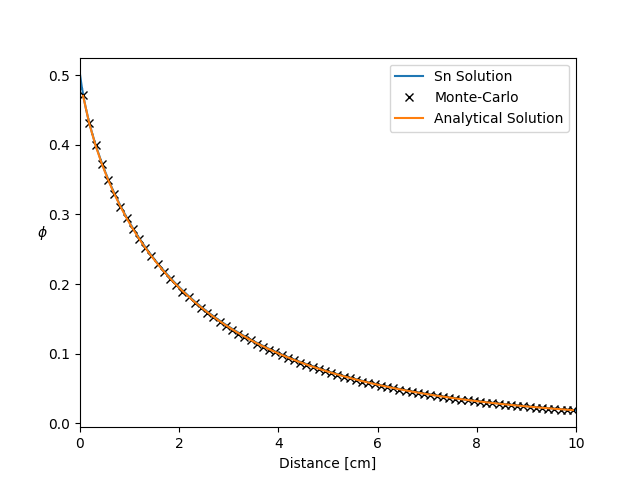
\includegraphics[width=0.7\linewidth]{images/Test_3_1}
\caption{Comparison of numerical Sn solution. The material for this problem was $\Sigma_t=0.2$, $\Sigma_s=0$ and a unity incident isotropic flux.}
\label{fig:Test_3_1}
\end{figure}


\subsection{Boundary incident isotropic flux}

\beq
\psi(\mu) = \frac{\phi}{2}
\eeq 

\beq
\int_{0}^{1} \mu \Psi(\mu).d\mu &= \int_{0}^{1} \mu \frac{\phi}{2} .d\mu \\
&= \frac{\phi}{2} \int_{0}^{1} \mu.d\mu \\
&= \frac{\phi}{2} \biggr[ \frac{1}{2}\mu^2 \biggr]_{0}^{1}
&= \frac{\phi}{4}
\eeq 






\newpage
\section{Diffusion Synthetic Acceleration (DSA)}
We can derive the diffusion equation from the transport equation by taking the first and second moment expansions of the transport equation resulting in the well known diffusion equation

\beqn \label{eq:diffusionEquation}
-\nabla D_g \nabla \phi_g+ \Sigma_{rg} \phi_g = 
\sum_{\substack{g'=0 \\ g'\ne g}}^{G-1} \Sigma_{s,g' \to g} \phi_{g'} + q_g
\eeqn 

We multiply by the weight function $\varphi_i$ and integrate over the volume 

\beq
-\int_V \varphi_i \nabla D_g \nabla \phi_g.dV+ \int_V \varphi_i \Sigma_{rg} \phi_g.dV = 
\sum_{\substack{g'=0 \\ g'\ne g}}^{G-1} \int_V \varphi_i \Sigma_{s,g' \to g} \phi_{g'}.dV + \int_V \varphi_i q_g.dV
\eeq

We then apply integration by parts on the first term

\beq
-\int_V \nabla (\varphi_i. D_g \nabla \phi_g).dV + \int_V ( \nabla \varphi_i ) (D_g \nabla \phi_g).dV
+ \int_V \varphi_i \Sigma_{rg} \phi_g.dV = 
\sum_{\substack{g'=0 \\ g'\ne g}}^{G-1} \int_V \varphi_i \Sigma_{s,g' \to g} \phi_{g'}.dV + \int_V \varphi_i q_g.dV
\eeq

and then apply Gauss' Divergence Theorem

\beqn \label{eq:diffusionbeforebasis}
&-\int_S \hat{n} \cdot (\varphi_i. D_g \nabla \phi_g).dA \\
&+ \int_V ( \nabla \varphi_i ) (D_g \nabla \phi_g).dV
+ \int_V \varphi_i \Sigma_{rg} \phi_g.dV = 
\sum_{\substack{g'=0 \\ g'\ne g}}^{G-1} \int_V \varphi_i \Sigma_{s,g' \to g} \phi_{g'}.dV + \int_V \varphi_i q_g.dV
\eeqn

We now expand our unknown flux $\phi$ into basis functions

\beq 
\phi \approx \phi_r = \sum_{j=0}^{J_k-1} \phi_j b_j
\eeq 

and then insert it into the weak form

\beq
&-\sum_{j=0}^{J_k-1} \int_S \hat{n} \cdot (\varphi_i. D_g \phi_{gj}\nabla b_j ).dA \\
&+ \sum_{j=0}^{J_k-1} \int_V ( \nabla \varphi_i ) (D_g \phi_{gj} \nabla b_j).dV
+ \sum_{j=0}^{J_k-1} \int_V \varphi_i \Sigma_{rg}\phi_{gj}b_j.dV = 
\sum_{j=0}^{J_k-1} \sum_{\substack{g'=0 \\ g'\ne g}}^{G-1} \int_V \varphi_i \Sigma_{s,g' \to g} \phi_{g'j}b_j.dV + \int_V \varphi_i q_g.dV
\eeq

Rearranging spatially dependent terms we get

\beqn \label{eq:FEMdiffusion}
&-\sum_{j=0}^{J_k-1} \int_S \hat{n} \cdot D_g \phi_{gj}(\varphi_i. \nabla b_j ).dA \\
&+ \sum_{j=0}^{J_k-1} \biggr( D_g  \int_V ( \nabla \varphi_i ) ( \nabla b_j).dV \biggr) \phi_{gj}
+ \sum_{j=0}^{J_k-1} \biggr( \Sigma_{rg}\int_V \varphi_i b_j.dV \biggr) \phi_{gj} \\
&= 
\sum_{j=0}^{J_k-1} \sum_{\substack{g'=0 \\ g'\ne g}}^{G-1} \biggr( \Sigma_{s,g' \to g}   \int_V \varphi_i b_j.dV \biggr) \phi_{g'j} +q_g\int_V \varphi_i .dV
\eeqn

The choice now is to use either a Continuous Finite Element Method (CFEM) approach or a Discontinuous Finite Element Method (DFEM) approach. For the CFEM we have the problem that the transport sweeps have been done with a DFEM and therefore jumps may exist at the boundaries of each element that would not exist in the CFEM case. For consistency we therefore use a DFEM approach here too, however, this requires special treatment of the surface integral. 

\vspace{0.5cm}
\textbf{A step back}\newline
Let us consider the diffusion equation before we expanded $\phi$ into bases. Let us remove the subscript $g$, lump the entire right hand side terms into a fixed source $s$ and remove the absorbtion term to get a simplified version

\beqn \label{eq:simplediffusion}
 \int_V ( \nabla \varphi_i ) ( \nabla \phi).dV 
 -\int_S \hat{n} \cdot (\varphi_i. D \nabla \phi).dA 
 = 
\int_V \varphi_i s.dV
\eeqn
\newline
We now define two terms that have a number of unknowns but which we will develop further. First we assume the variable of interest $\phi$ to be discontinuous on the boundary of the element. For simplicity consider any boundary between two elements in a 1D sense. Denote the function on the element to the left with a negative sign $\phi_i^-$ and on the right with $\phi_i^+$. Next we define the average of these two quantities on the boundary. Now, it seems in many mathematical papers the convention is to use double curly braces for the average and block brackets for the jump. Hence we have the average as

$$
\{\{ \phi  \}\} = \frac{\phi^- + \phi^+}{2}
$$

and the jump as 
$$
[[ \phi ]] = \phi^+ - \phi^-
$$
\newline
We now replace the normal derivative with

\beqn \label{eq:interfacecurrents}
-\int_S \hat{n} \cdot (\varphi_i. D \nabla \phi).dA  
&=-\int_S \varphi_i \biggr( \alpha [[ \phi ]] + \hat{n}\cdot D \nabla \{\{ \phi  \}\} \biggr).dA \\
&=-\int_S \varphi_i \biggr( 
(\alpha \phi^+ + \hat{n}\cdot D \nabla \phi^+) 
 -(\alpha \phi^- - \hat{n}\cdot D \nabla \phi^-)
\biggr).dA \\
&=\int_S \varphi_i \biggr( 
(\alpha \phi^- - \hat{n}\cdot D \nabla \phi^-)
-(\alpha \phi^+ + \hat{n}\cdot D \nabla \phi^+) 
\biggr).dA
\eeqn
\newline
It is important to note that $\phi^-$ is always within the cell and $\phi^+$ is always in the adjacent cell. With this scheme we can again expand the variables of interest into basis functions taking care to note that the basis functions used for $\phi^+$ is that of the adjacent element. We have not yet defined the coefficient $\alpha$ and in many references it is loosely defined as $\alpha=\frac{1}{4}$, however, when considering angular flux this coefficient becomes apparent, i.e. suppose we have an isotropic flux $\phi$. The angular flux $\Psi$ is given by

\beq 
\Psi(\Omega)= \frac{\phi}{4\pi}
\eeq 
\newline
Now taking the dot product with a surface normal we essentially transform the current onto a new angle orientation $\Omega'$ for which we can integrate over the shifted azimuthal

\beq 
\Psi(\mu)= \frac{\phi}{2} 
\quad \quad \text{ and } \quad \quad
J(\mu) =  \mu \frac{\phi}{2}
\eeq 

And then 

\beq
J^{+} &= \frac{\phi}{2} \int_{1}^{0} \mu.d\mu \\
&=\frac{\phi}{4}
\eeq
\newline
The effective incoming current is the difference of the outgoing current within the element and the outgoing current of the adjacent element. Therefore using $\alpha=\frac{1}{4}$ is an appropriate choice.

\vspace{0.5cm}
\textbf{Back to the Finite Elements} \newline
We now insert equation \ref{eq:interfacecurrents} into equation \ref{eq:FEMdiffusion} to get

\beqn \label{eq:DGDiffusion}
&\sum_{j=0}^{J_k -1} 
\biggr(
 \int_{S} \varphi_i \biggr[
 \alpha - \hat{n}_k\cdot D_g.\nabla b_j
\biggr] .dA 
\biggr) \phi_j^-
+
\sum_{j=0}^{J_k^- -1} 
\biggr(
 \int_{S^-} \varphi_i \biggr[
 -\alpha - \hat{n}_k\cdot D_g.\nabla b_j
\biggr] .dA 
\biggr) \phi_j\\
&+ \sum_{j=0}^{J_k-1} \biggr( D_g  \int_V ( \nabla \varphi_i ) ( \nabla b_j).dV \biggr) \phi_{gj}
+ \sum_{j=0}^{J_k-1} \biggr( \Sigma_{rg}\int_V \varphi_i b_j.dV \biggr) \phi_{gj} \\
&= 
\sum_{j=0}^{J_k-1} \sum_{\substack{g'=0 \\ g'\ne g}}^{G-1} \biggr( \Sigma_{s,g' \to g}   \int_V \varphi_i b_j.dV \biggr) \phi_{g'j} +q_g\int_V \varphi_i .dV
\eeqn

\newpage
\subsection{Within Group DSA} 
The diffusion equation depicted in equation \ref{eq:DGDiffusion} cannot be used to replace the transport iterations in this form since it will attempt to replace the more accurate transport estimate with that of an isotropic diffusion estimate, however, it can be used to accelerate the within group scattering source by employing the scheme as depicted here. We start by computing the inscattering source term for equation \ref{eq:NTEoperatorform} at iteration $(\ell)$ and use it to compute the solution of the angular flux at iteration $\ell+\ell_{T}$, where $\ell_T$ refers to the angular flux estimate after a single transport sweep

\beq
\mathbf{L \Psi^{(\ell + \ell_T)}} &= \mathbf{MSD\Psi^{(\ell)}} + \mathbf{S} \\
&=\mathbf{MS\Phi^{(\ell)}} + \mathbf{S} \\
&\text{and}\\
\mathbf{\Phi^{(\ell+\ell_T)}} &= \mathbf{D\Psi^{(\ell+\ell_T)} }
\eeq 
\newline
We then define the change in the zeroth flux moment (i.e. the scalar flux) as

\beq
F_{0g}^{(\ell+\ell_T)} &=    \phi_{0g}^{(\ell + \ell_T)} - \phi_{0g}^{(\ell )} \\
F_{0g}^{(\ell+\ell_W)} &=    \phi_{0g}^{(\ell + \ell_W)} - \phi_{0g}^{(\ell )} \\
\eeq 
where $\ell_W$ is the iteration step after within-group acceleration and we note that after manipulating the diffusion equation we get

\beqn
-\frac{\partial }{\partial x} D_g \frac{\partial F_{0g}}{\partial x}^{(\ell+\ell_W)}  
+ \quad \Sigma_{rg} F_{0g}^{(\ell+\ell_W)}
=
\Sigma_{s0,g{\to}g} F_{0g}^{(\ell+\ell_T)}
\eeqn 

we then apply the finite element discretization previously discussed, equation \ref{eq:DGDiffusion}, 

\beqn
&\sum_{j=0}^{J_k -1} 
\biggr(
 \int_{S} \varphi_i \biggr[
 \alpha - \hat{n}_k\cdot D_g.\nabla b_j
\biggr] .dA 
\biggr) F_{0gj}^{(\ell+\ell_W)-}
+
\sum_{j=0}^{J_k^- -1} 
\biggr(
 \int_{S^-} \varphi_i \biggr[
 -\alpha - \hat{n}_k\cdot D_g.\nabla b_j
\biggr] .dA 
\biggr) F_{0gj}^{(\ell+\ell_W)}  \\
&+ \sum_{j=0}^{J_k-1} \biggr( D_g  \int_V ( \nabla \varphi_i ) ( \nabla b_j).dV \biggr) F_{0gj}^{(\ell+\ell_W)} 
+ \sum_{j=0}^{J_k-1} \biggr( \Sigma_{rg}\int_V \varphi_i b_j.dV \biggr) F_{0gj}^{(\ell+\ell_W)}  \\
&= 
\sum_{j=0}^{J_k-1}  \biggr( \Sigma_{s0,g \to g}   \int_V \varphi_i b_j.dV \biggr) F_{0gj}^{(\ell+\ell_T)} 
\eeqn

The WGDSA effectively reduces the spectral radius from $>$0.98 to the a low 0.9 and hence there is still more to be done with the acceleration of up-scattering.


\newpage
\subsection{Two Grid Diffusion Synthetic Acceleration (TGDSA)}






\newpage
\section{Multigroup Test problem}

\begin{figure}[H]
\centering
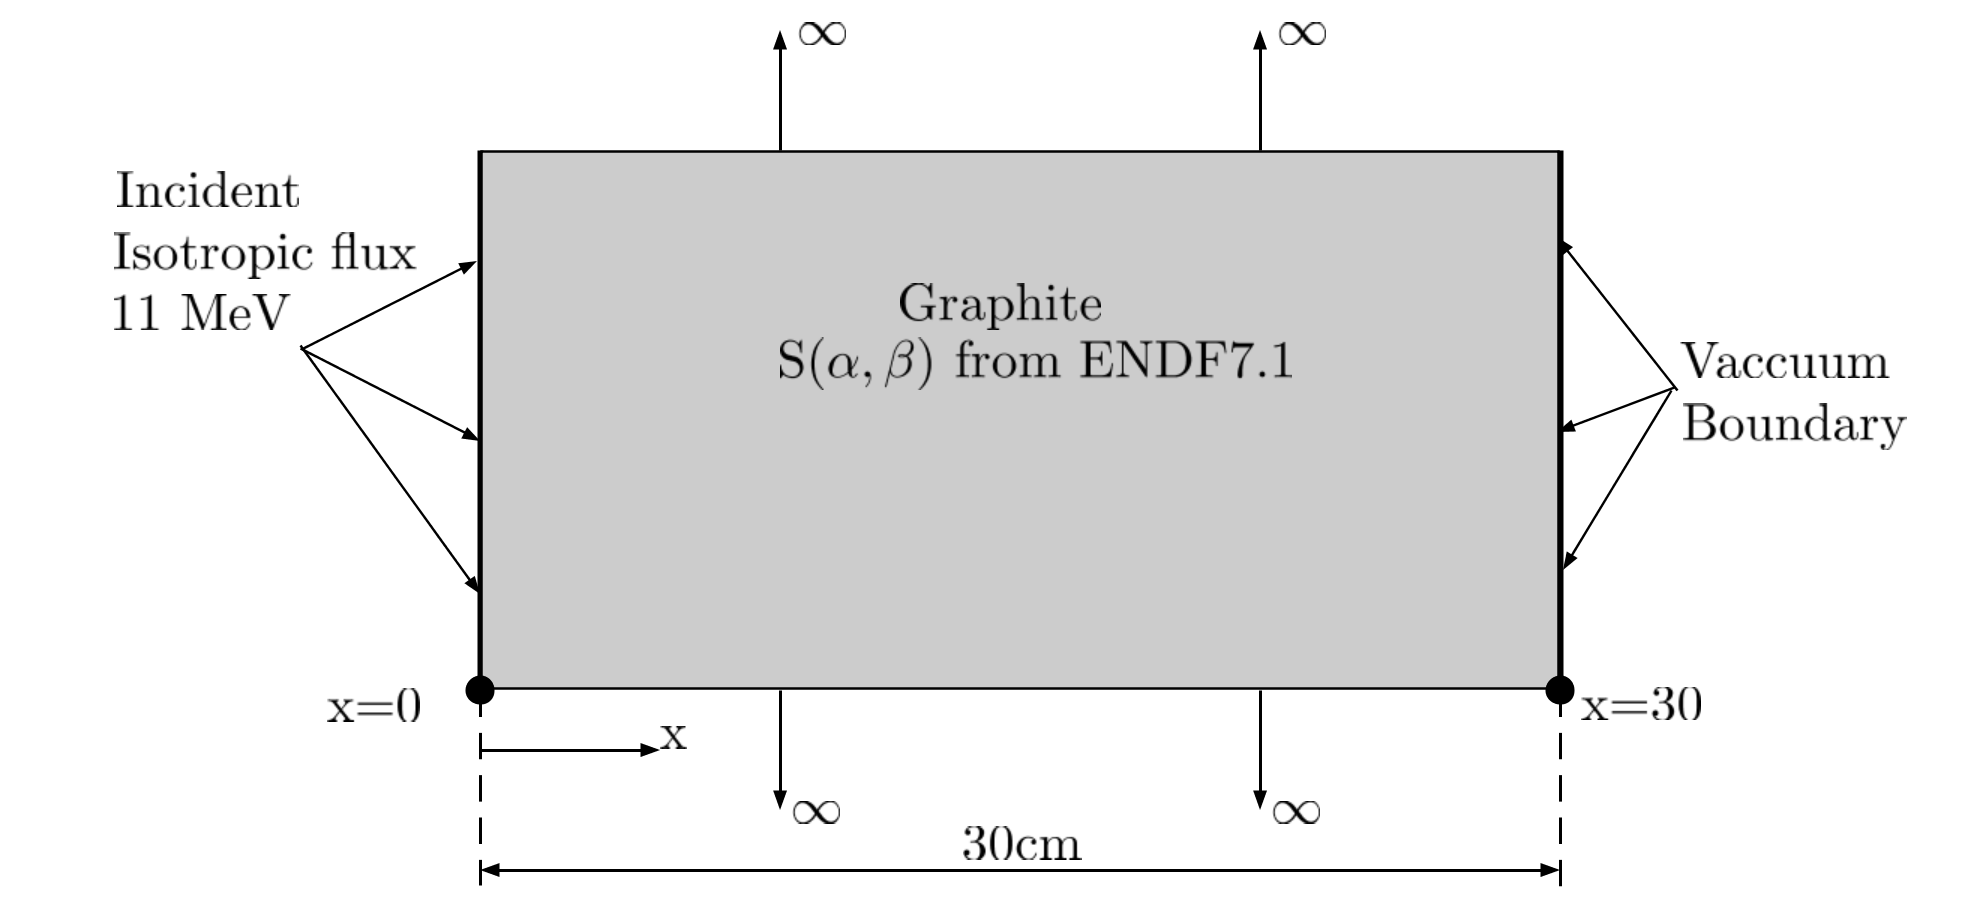
\includegraphics[width=0.8\linewidth]{images/MGProblem.png}
\caption{Multigroup test problem.}
\label{fig:MGProblem}
\end{figure}

Consider the infinite slab geometry depicted in Figure \ref{fig:MGProblem}. Using a fine resolution 168 energy group structure we can use different spatial resolutions, scattering orders and angular quadratures and compare the solution. As a first round of comparison we look at a comparison with MCNP in 




\newpage
\begin{appendices}
\section{Integral of the basis functions}
We start with the integral of $\varphi$

\beq
\int_{x_i}^{x_{i+1}} \varphi_i .dx &= \frac{x_{i+1}-x_i}{2} \int_{-1}^{+1} N_i .d\xi \\
\int_{x_i}^{x_{i+1}} \varphi_0 .dx &= \frac{x_{i+1}-x_i}{2} \int_{-1}^{+1} (-\frac{1}{2}\xi+\frac{1}{2}) .d\xi \\
&=  \frac{x_{i+1}-x_i}{4} \biggr[-\frac{1}{3}\xi^2 + \xi \biggr]_{-1}^{+1}\\
&=  \frac{x_{i+1}-x_i}{4} \biggr[\frac{2}{3} - (-\frac{4}{3}) \biggr]\\
&=\frac{x_{i+1}-x_i}{2}=\frac{h}{2}
\eeq 

\beq
\int_{x_i}^{x_{i+1}} \varphi_1 .dx &= \frac{x_{i+1}-x_i}{2} \int_{-1}^{+1} (+\frac{1}{2}\xi+\frac{1}{2}) .d\xi \\
&=  \frac{x_{i+1}-x_i}{4} \biggr[\frac{1}{3}\xi^2 + \xi \biggr]_{-1}^{+1}\\
&=  \frac{x_{i+1}-x_i}{4} \biggr[\frac{4}{3} - (-\frac{2}{3}) \biggr]\\
&=\frac{x_{i+1}-x_i}{2} = \frac{h}{2}
\eeq 

Then we do the integral of the product $\varphi_i.b_j$

\beq
\int_{x_i}^{x_{i+1}} \varphi_0 b_0.dx &= \frac{x_{i+1}-x_i}{2} \int_{-1}^{+1} (-\frac{1}{2}\xi+\frac{1}{2})(-\frac{1}{2}\xi+\frac{1}{2}) .d\xi \\
&=  \frac{x_{i+1}-x_i}{8} \int_{-1}^{+1} (-\xi +1 )(-\xi +1).d\xi \\
&=  \frac{x_{i+1}-x_i}{8} \int_{-1}^{+1} (\xi^2-2\xi+1 ).d\xi \\
&=  \frac{x_{i+1}-x_i}{8} \biggr[  \frac{1}{3}\xi^3 -\xi^2+\xi  \biggr]_{-1}^{+1}\\
&= \frac{x_{i+1}-x_i}{8} \biggr[  \frac{1}{3} - (-\frac{1}{3}-\frac{3}{3} -\frac{3}{3}) \biggr]\\
&=  \frac{x_{i+1}-x_i}{3} = \frac{h}{3}
\eeq 

\beq
\int_{x_i}^{x_{i+1}} \varphi_1 b_1.dx &= \frac{x_{i+1}-x_i}{2} \int_{-1}^{+1} (\frac{1}{2}\xi+\frac{1}{2})(\frac{1}{2}\xi+\frac{1}{2}) .d\xi \\
&=  \frac{x_{i+1}-x_i}{8} \int_{-1}^{+1} (\xi +1 )(\xi +1).d\xi \\
&=  \frac{x_{i+1}-x_i}{8} \int_{-1}^{+1} (\xi^2+2\xi+1 ).d\xi \\
&=  \frac{x_{i+1}-x_i}{8} \biggr[  \frac{1}{3}\xi^3 +\xi^2+\xi  \biggr]_{-1}^{+1}\\
&= \frac{x_{i+1}-x_i}{8} \biggr[  \frac{7}{3} - (-\frac{1}{3}+\frac{3}{3} -\frac{3}{3}) \biggr]\\
&=  \frac{x_{i+1}-x_i}{3} = \frac{h}{3}
\eeq 

\beq
\int_{x_i}^{x_{i+1}} \varphi_1 b_0.dx = 
\int_{x_i}^{x_{i+1}} \varphi_0 b_1.dx &= \frac{x_{i+1}-x_i}{2} \int_{-1}^{+1} (-\frac{1}{2}\xi+\frac{1}{2})(+\frac{1}{2}\xi+\frac{1}{2}) .d\xi \\
&=  \frac{x_{i+1}-x_i}{8} \int_{-1}^{+1} (-\xi +1 )(\xi +1).d\xi \\
&=  \frac{x_{i+1}-x_i}{8} \int_{-1}^{+1} (-\xi^2+1 ).d\xi \\
&=  \frac{x_{i+1}-x_i}{8} \biggr[  -\frac{1}{3}\xi^3 +\xi  \biggr]_{-1}^{+1}\\
&= \frac{x_{i+1}-x_i}{8} \biggr[  \frac{2}{3} - (\frac{1}{3} -\frac{3}{3}) \biggr]\\
&=  \frac{x_{i+1}-x_i}{6} = \frac{h}{6}
\eeq 

And finally the integral of $\varphi_i.\frac{\partial b_j}{\partial x}$

\beq
\int_{x_i}^{x_{i+1}} \varphi_0.\frac{\partial b_0}{\partial x}.dx 
&= -\frac{1}{4}\int_{-1}^{+1} (-\xi +1).d\xi \\
&=-\frac{1}{4} \biggr[ -\frac{1}{2}\xi^2 + \xi   \biggr]_{-1}^{+1}\\
&=-\frac{1}{4} \biggr[ \frac{1}{2} - (- \frac{1}{2} -\frac{2}{2})  \biggr] \\
&=-\frac{1}{2}
\eeq 

\beq
\int_{x_i}^{x_{i+1}} \varphi_1.\frac{\partial b_1}{\partial x}.dx 
&= \frac{1}{4}\int_{-1}^{+1} (\xi +1).d\xi \\
&=\frac{1}{4} \biggr[ \frac{1}{2}\xi^2 + \xi   \biggr]_{-1}^{+1}\\
&=\frac{1}{4} \biggr[ \frac{3}{2} - ( \frac{1}{2} -\frac{2}{2})  \biggr] \\
&=\frac{1}{2}
\eeq 

\beq
\int_{x_i}^{x_{i+1}} \varphi_0.\frac{\partial b_1}{\partial x}.dx 
&= \frac{1}{4}\int_{-1}^{+1} (\xi +1).d\xi \\
&=\frac{1}{4} \biggr[ \frac{1}{2}\xi^2 + \xi   \biggr]_{-1}^{+1}\\
&=\frac{1}{4} \biggr[ \frac{3}{2} - (\frac{1}{2} -\frac{2}{2})  \biggr] \\
&=\frac{1}{2}
\eeq 

\beq
\int_{x_i}^{x_{i+1}} \varphi_1.\frac{\partial b_0}{\partial x}.dx 
&=-\frac{1}{4}\int_{-1}^{+1} (-\xi +1).d\xi \\
&=-\frac{1}{4} \biggr[ -\frac{1}{2}\xi^2 + \xi   \biggr]_{-1}^{+1}\\
&=-\frac{1}{4} \biggr[ \frac{1}{2} - ( -\frac{1}{2} -\frac{2}{2})  \biggr] \\
&=-\frac{1}{2}
\eeq     

We also have the integral of the product of $\frac{\partial \varphi_i}{\partial x}.\frac{\partial b_j}{\partial x}$

\beq
\int_{x_i}^{x_{i+1}}\frac{\partial \varphi_0}{\partial x}.\frac{\partial b_0}{\partial x}.dx 
&= \frac{x_{i+1}-x_i}{2} \frac{2}{x_{i+1}-x_i} \frac{2}{x_{i+1}-x_i} \int_{-1}^{+1} (-\frac{1}{2})(-\frac{1}{2}).d\xi \\
&= \frac{2}{x_{i+1}-x_i} \int_{-1}^{+1} \frac{1}{4}.d\xi \\
&= \frac{2}{x_{i+1}-x_i} \biggr[ \frac{1}{4}\xi \biggr]_{-1}^{+1} \\
&= \frac{1}{h}
\eeq 

\beq
\int_{x_i}^{x_{i+1}}\frac{\partial \varphi_0}{\partial x}.\frac{\partial b_1}{\partial x}.dx 
&= \frac{x_{i+1}-x_i}{2} \frac{2}{x_{i+1}-x_i} \frac{2}{x_{i+1}-x_i} \int_{-1}^{+1} (-\frac{1}{2})(\frac{1}{2}).d\xi \\
&= -\frac{1}{h}
\eeq 

\beq
\int_{x_i}^{x_{i+1}}\frac{\partial \varphi_1}{\partial x}.\frac{\partial b_0}{\partial x}.dx 
&= \frac{x_{i+1}-x_i}{2} \frac{2}{x_{i+1}-x_i} \frac{2}{x_{i+1}-x_i} \int_{-1}^{+1} (\frac{1}{2})(-\frac{1}{2}).d\xi \\
&= -\frac{1}{h}
\eeq     

\beq
\int_{x_i}^{x_{i+1}}\frac{\partial \varphi_1}{\partial x}.\frac{\partial b_1}{\partial x}.dx 
&= \frac{x_{i+1}-x_i}{2} \frac{2}{x_{i+1}-x_i} \frac{2}{x_{i+1}-x_i} \int_{-1}^{+1} (\frac{1}{2})(\frac{1}{2}).d\xi \\
&= \frac{1}{h}
\eeq    
    
\end{appendices}

\newpage
\chead{References}
\begin{thebibliography}{1}
    
    \bibitem{roots} Barrera-Figueroa V., et al. {\em Multiple root finder algorithm for Legendre and Chebyshev polynomials via Newton’s method}, Annales Mathematicae et Informaticae, volume 33, pages 3-13, 2006
    
    
\end{thebibliography}

    
    
    
    
\end{document}
